\documentclass{article}
\usepackage[utf8]{inputenc}
\usepackage[margin =1.25in,includefoot]{geometry}
\usepackage{indentfirst}
\usepackage{graphicx}
\usepackage{float}

\title{COP290 Maze-Simulation}
\date{May 2021}
\author{Aniket Gupta \hspace{2cm}  Aayush Goyal \\
    2019CS10327 \hspace{2.3cm} 2019CS10452}

\begin{document}

\maketitle

\section{Problem statement}
A new Pizza-Hut has opened in a city and it needs to deliver some orders. There is a lot of traffic in the city, so the members of that city often face the problem of getting late deliveries. To make profits this Pizza-Hut offers a scheme that they will deliver the Pizza in some time limit else they will get the order for free. The Pizza-Hut owner hired you to make an App that shows the delivery guy a delivery location such that it is closest to it's current location. So we have to use some algorithm and also simulate the path to be taken to reach that point in minimum time.
\\
\par Mathematically we have to start from a point in the Maze, and then reach fixed set of points one by one as soon as possible.

\\\\
\subsection{City Map} 

\begin{figure}[H]
     \centering
     \subfigure{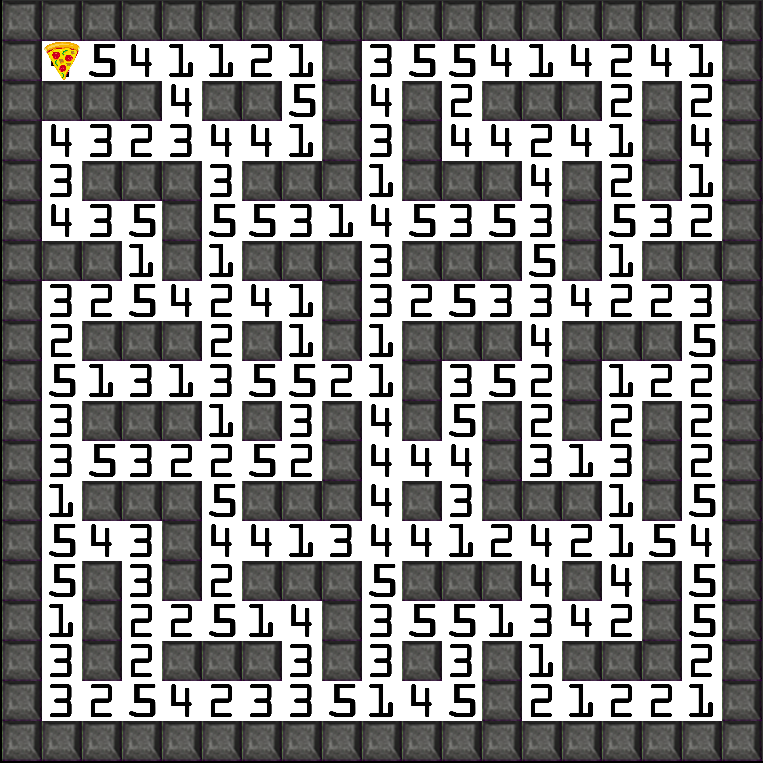
\includegraphics[width=9cm,height=9cm \textwidth]{images/simMaze.PNG}} 
\end{figure}
The Delivery-man has the map of the city. So, he/she can decide before-hand the path to travel. This decision takes time. The simulation shows this decision making process as well as the final path taken. The Delivery guy will follow that path to go to the desired location.
\\
\par
\textbf{Note:} For building the maze in this subtask, we modified the maze algorithm that we used in the subtask-1 of Assignment-2 (COP290).

\subsection{Description of the City Map}
The city is represented as a N \textbf{x} M matrix. Different cells in the map represent different locations in the city. The different parts in the city have different traffics, road-quality etc. Thus, it takes different amount of times to travel different locations in the city. This time is shown in the matrix by assigning some weight to each cell. For example, if X is a cell with $W_X$ as its weight, then it takes $W_X$ amount of time to reach X from any of its adjacent cells.

\section{Approach and Algorithm}
To solve this problem algorithmically, the entire city can be thought of as a graph where each location shown in the map is considered a graph vertex and adjacent locations are connected by directed edges. For example, if X and Y are adjacent locations with weight $W_X$ and $W_Y$ respectively, then the edge from X to Y has weight $W_Y$ and that from Y to X has weight $W_X$.
\\\\
Starting from the initial location, we first find the delivery location that takes least time to reach from initial location. To do so, we use the Dijkstra's algorithm. Note that Dijkstra's algorithm gives the smallest distance (distance here means the sum of weights of edges in the path) from staring node to all the nodes in the graph. \textbf{But, to find the nearest delivery location, we don't need to find the minimum distance to all the nodes. We stop the algorithm as soon as the first delivery point is found}. This will be the nearest delivery location from the staring point (as proved below). After reaching the first delivery point, again start the algorithm with this delivery location as the starting point and find the nearest unvisited delivery point from this location. Keep repeating this until all the delivery points are covered.
\\\\
\textbf{Note}: In the entire document, whenever we say smallest path, it means the path that takes minimum amount of time to reach destination from current location.

\section{Dijkstra's Algorithm}

\subsection{Mechanism}
In Dijkstra's algorithm, we start with an initial node whose distance to itself is zero, and distance to all others is $\infty$. We maintain 2 sets- VISITED and UNVISITED. The first set (VISITED) contains the nodes for which the shortest distance from starting node has been found. For each node in the VISITED set, we also store the shortest distance from the starting node. The second set (UNVISITED) contains the nodes for which the shortest distance is yet to be found. In the UNVISITED set, for the nodes which have an edge with atleast one vertex in the VISITED set, we store the length of smallest path that starts at the starting point and ends at the current node and has all the other vertices belonging to the VISITED set. For other nodes in UNVISITED set, their distance from first node is stored as $\infty$. 
\\
\par Initially, only the starting node is stored in the VISITED set with distance zero. During each iteration in the algorithm, we select a node from the UNVISITED set with smallest distance and move it in VISITED set. When a node is moved from UNVISITED to VISITED set, all its neighbouring nodes' distances that are still in the UNVISITED set is updated if the distance gets reduced. This is repeated until the UNVISITED set becomes empty.

\subsection{Correctness of Algorithm in searching the nearest Delivery Point}\\\\
Dijkstra's algorithm gives the minimum distance of all nodes from the starting point. We are using the fact that the first delivery point that is reached during the algorithm is the nearest delivery point.
\\\\
\textbf{To Prove:} 
The first delivery point (among all the remaining delivery points) whose distance is found first during the Dijkstra's algorithm is the nearest delivery point from the starting position.
\\\\
\textbf{Proof:} To prove this statement, we use the following lemma.\\
\textbf{Lemma:} The nodes are inserted in the VISITED set (i.e., processed) in the order of increasing minimum distance from the starting node.
\\
\noindent\rule{\textwidth}{0.4pt}
\textbf{Proof for the lemma} -
We will prove this using Strong Induction
\\\\
\textbf{Induction Hypothesis:}\\
If we have processed $n$ nodes in the order, say $a_1, a_2, ...., a_n$ in the Dijkstra's algorithm then $dist[a_1] \le dist[a_2] \le ... \le dist[a_n] $
\\\\
\textbf{Base case:}\\
When the starting node is processed, the distance of all the other nodes is $\infty$. Then we reduce their distance using the edges that go out from starting point. Now since every edge length is positive so the next point that we will select, its distances would be more than the starting node. All these nodes are inserted in the priority queue and the one with least distance is selected. Hence the induction hypothesis is true for n= 1, 2.
\\\\
\textbf{Induction step:}\\
Now we will select the $(n+1)^{th}$ node from the priority queue. The node with the least distance would be selected. If $a_{n+1}$ is present in the priority queue then it must have come through some previously visited point, say $a_m$. Now since all the edges are of positive length, we can say that $dist[a_{n+1}] \ge dist[a_m]$. Now let us say that there exists a node $a_k$ such that $dist[a_k] > dist[a_{n+1}]$. Now 3 cases are possible:
\begin{itemize}
    \item k$>$ m: If k$>$ m, then from the Induction hypothesis we have $dist[a_{k}] \ge dist[a_m]$. Now after the $m^{th}$ selection we had $a_{n+1}$ also present in the priority queue. If $dist[a_k] \ge dist[a_{n+1}]$ then according to the rule we would have selected $a_{n+1}$ before $a_k$. So k$>$ m is not possible.
    \item k$<$ m: If k$<$ m, then from the Induction hypothesis we have $dist[a_{m}] \ge dist[a_k]$. Also we shown that $dist[a_{n+1}] \ge dist[a_m]$. So k$<$ m is not possible.
    \item k$=$ m: This is also not possible since there are no negative edges.
\end{itemize}
Hence such a $k$ doesn't exist and $dist[a_{n+1}]$ is greater than or equal to the distances of nodes inserted before it. Thus the induction hypothesis is also true for $n+1$. Thus the lemma is correct.
\par\noindent\rule{\textwidth}{0.4pt}
\\\\
Now, the above lemma shows that the nodes are put in the VISITED set in increasing order of minimum distance from the starting node. Thus, the first delivery point that is put in the VISITED set would have smaller (or equal) distance than the delivery points that are still waiting to be put in the VISITED set. This completes our proof that the first delivery point (among all the remaining delivery points) whose distance is found during the Dijkstra's algorithm is the nearest delivery point from the starting position.




\subsection{Runtime Analysis}
A constraint for using Dijkstra's algorithm is that there must not be any negative edge in the graph. We process every edge once, using the fact there are no negative edges and this is the reason why it gives better efficiency than Bellman-Ford Algorithm. In Dijkstra's algorithm whenever a node is selected (put into VISITED set), it's shortest distance from the starting node is final. We are iterating through every directed edge only once and every edge has the tendency to enter in the binary heap (since we are not updating priority, instead adding another element). Also every node is processed only once. Thus the complexity of Dijkstra's algorithm is $O(n + m\log m)$, $n$ is number of nodes and $m$ is no. of edges in the graph.
\\
\par If there are $k$ delivery points, then we will have to run the Algorithm each time, with a new start point. We stop the algorithm once we find any such unvisited delivery point. 
\\
\par Let the Height and Width be $n$ and $m$, no. of delivery points be $k$. No. of nodes in the graph can be at m$n*m$ and no. of edges in the graph can be at max $4*n*m$. Thus the overall time complexity would be \textbf{$O(k*nm*\log nm)$}.

\subsection{Data Structures}

\subsubsection{Binary Min Heap}
The efficient implementation of Dijkstra's algorithm requires that we are able to update the priority of the Every Node of the graph. Also we must be able to extract the Node with highest priority as soon as possible.
\\
\par Binary Min-heap or a Priority Queue are very efficient data structures to serve this purpose.
\begin{enumerate}
    \item \textbf{Top priority element:}  Binary heap is built in such a way that the element with the top priority remains at the top as the root of the tree. So we need to keep a pointer to the root node of the binary heap. Time Complexity for this would be $O(1)$. 
    \item \textbf{Adding element}: The Time required to add any element in the Binary heap is $O(\log_2 N)$, where N is the size of Queue.
    \item \textbf{Updating Priority}: Updating Priority is done by re-adding that node with the new priority in the Binary heap. A remarkable property of the Dijkstra's algorithm is that whenever a node is selected it's distance is final. So we keep a Processed array to keep track of all the selected nodes. Whenever the Priority Queue returns the same node again we reject it because it was once already processed. In this way updating the priority can be done in same $O(\log_2 N)$ time.
    \\\\
    \textbf{Note:} We have to re-add the element because we cannot search for the already existing node and update it's priority. Binary heaps are a very poor data structure if one intends to do searching of elements.
\end{enumerate}

\subsubsection{Balanced Binary Search Trees}
After each iteration of Dijkstra's algorithm we get a node. The shortest distance to that node from the starting node gets fixed. Now we need to check if it is one of the delivery points or not. To check this fastly we will need a Binary search tree. This will help us in completing the search in $O(\log_2 N)$ time.

\subsubsection{Adjacency List}
We don't want to waste time on checking if a node is connected to the given node or not. So for this we make an adjacency list from the the Maze. This adjacency list tells us the nodes reachable from one node and time (or weight) that would be required to go from $node_1$ to $node_2$. This would also make sure O(degree of node) time is spent on each node.

\section{Simulation}
\subsection{Selecting the Delivery Locations}
First the user gives the no. of delivery locations through terminal. Then, the city map appears on the window. User can then select the delivery locations using mouse. Every location you select gets marked in red. Choosing same location multiple times is counted only once. Walls are not a valid delivery location. Pizza denotes the starting location (location of Pizza-Hut, this is also an invalid delivery location)
\begin{figure}[H]
     \centering
     \subfigure{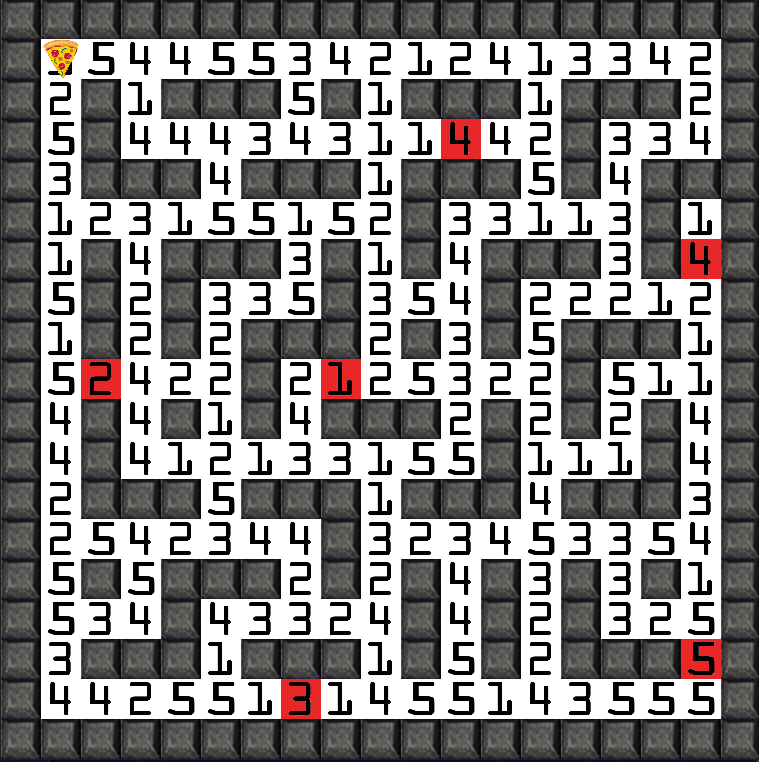
\includegraphics[width=8cm,height=8cm \textwidth]{images/simSelectingLocations.PNG}} 
\end{figure}

\subsection{Finding the nearest delivery location from the current location}
After the delivery locations are selected, the Dijkstra's algorithm tries to find the nearest delivery location. The locations whose least time to reach from the current starting location is already found are turned orange. The Dijkstra's searching method is stopped as soon reach time to some delivery point is found. This point will take the least amount of time to reach from the current location of Delivery boy (shown by Pizza slice).
\begin{figure}[H]
     \centering
     \subfigure{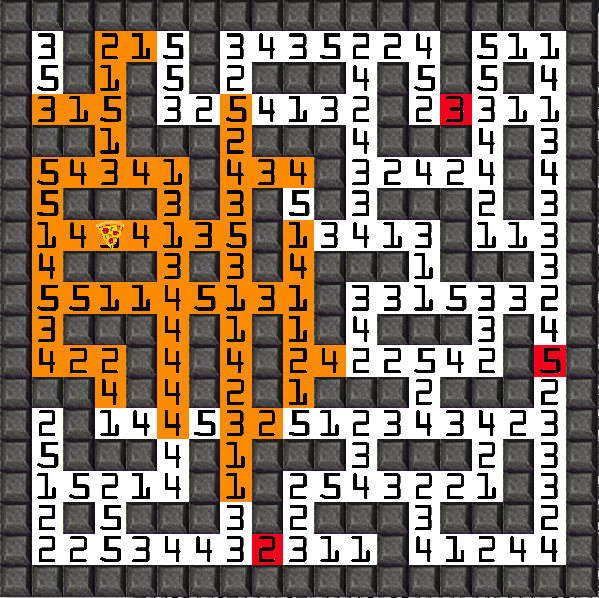
\includegraphics[width=9.5cm,height=9.5cm \textwidth]{images/simSearch.PNG}} 
\end{figure}

\subsection{Tracing back the optimal path}

During searching the nearest delivery point using the Dijkstra's algorithm, we kept storing the parent of each node (i.e. the neighbouring cell through which the shortest path from the starting location to current location passes). Once the nearest delivery location is found from the current location, the path is traced backed by starting a pointer at the delivery location and moving the pointer to the parent of the location pointed by the pointer. Keep repeating this step until the pointer reaches the starting location. Path will get highlighted in green color as we backtrack it.
\begin{figure}[H]
     \centering
     \subfigure{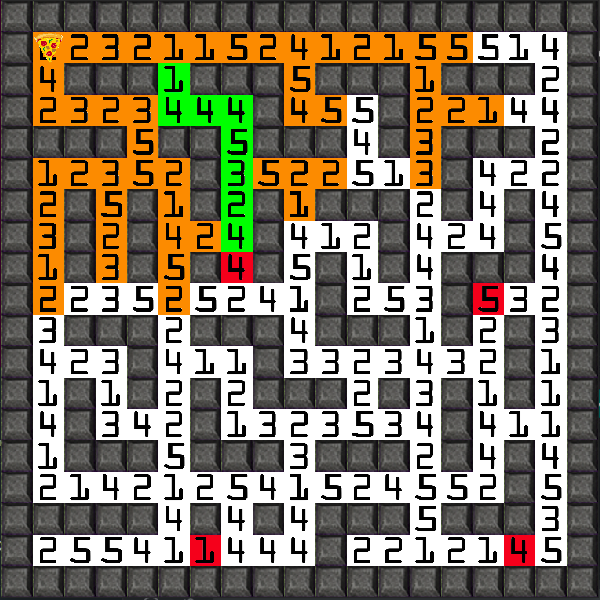
\includegraphics[width=8.5cm,height=8.5cm \textwidth]{images/simBacktrack.PNG}} 
\end{figure}

\subsection{Travelling at the path found}
Once the path is found from current location to the nearest delivery point, the delivery man travel this path to reach this destination. This is shown as a slice of pizza moving on the path. Pointy edge of Pizza slice shows the direction of movement.
\begin{figure}[H]
     \centering
     \subfigure{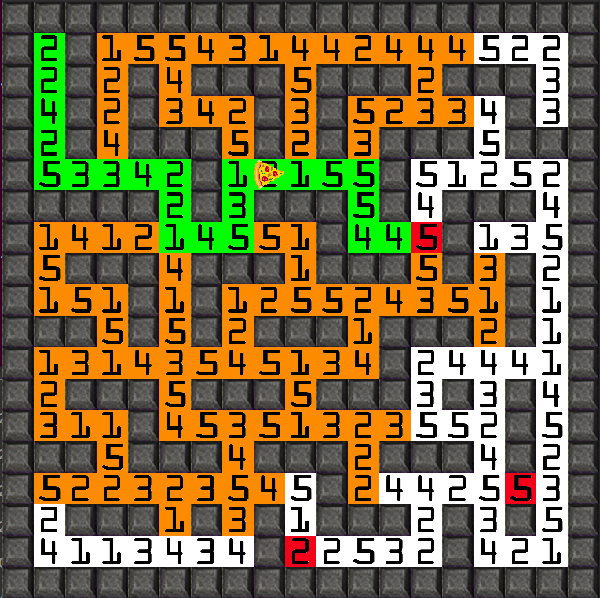
\includegraphics[width=8.5cm,height=8.5cm \textwidth]{images/simPathTrace.PNG}} 
\end{figure}

\subsection{Selecting next delivery point}
Once the current delivery point is reached, the Dijkstra's algorithm is ran again with this location as the starting point. It searches for the next delivery location that is nearest from the current location. This step is repeated until all the delivery points are covered.

\section{Visual affects added in the simulation}
To make the simulation visually appealing and aesthetic, we added the following features:
\begin{itemize}
\item While the nearest delivery point is being searched, the cells visited are shown in orange color.
\item To trace the path between the current location and the nearest delivery point, the cells are coloured green.
\item To show the movement of the delivery man, we show a slice of pizza moving from the starting point to the destination, with pointy end in the direction of moving.
\item We have added delay of around 100ms between selection of two cells to make the searching and traversal process visually attractive.
\end{itemize}
\section{Possible future improvements}
Currently, we are finding the nearest unvisited delivery point from current location (starting point or some already reached delivery point). What if two unvisited delivery points take same amount of time to reach from the current location? One possible improvement is whenever we find multiple delivery points that take equal time to reach, then instead of chosing one randomly, find the delivery point among them which, if taken, will give the nearest next delivery point (if there is one). Note that in our method, we are finding the nearest delivery point from the starting point and all but one (which is visited last) delivery points. Now, to chose among delivery points which take equal time to reach, if we run Dijkstra's algorithm from some delivery point and that node is not chosen as the next destination delivery point, then store the distances of the locations (for which the distance is already calculated) from this delivery point. And later when the nearest delivery point from this location is required, then use these already calculated distances from this location. Thus, the space complexity will increase but the time taken to deliver pizza will decrease.
\\






\end{document}
